\documentclass{article}
\usepackage[utf8]{inputenc}

\usepackage{amssymb}
\usepackage{amsmath}
\usepackage{float}
\usepackage[toc,page]{appendix}
\usepackage{listings}
\usepackage{geometry}
\geometry{
a4paper,
top=1in
}

\DeclareMathOperator{\Var}{Var}
\DeclareMathOperator{\Corr}{Corr}
\DeclareMathOperator{\Cov}{Cov}

\title{Time Series Project 2}
\author{Stefan Eng and Franz Hartleitner}
\date{May 2019}

\usepackage{natbib}
\usepackage{graphicx}

\begin{document}

\maketitle

\section*{Problem 1}

We computed the log returns $X_t = \log(P_t) - \log(P_{t - 1})$.
Using Matlab's Ljung-Box test \textit{lbqtest} with a lag $h = 20$, we got a p-value of 0.1331.
We fail to reject the null hypothesis at the $\alpha = 0.05$ significance level and conclude that the data in consistent with being $iid$.
In Figure \ref{fig:acf_log_rtns} we plot the autocorrelation function for the log returns.


\begin{figure}[H]
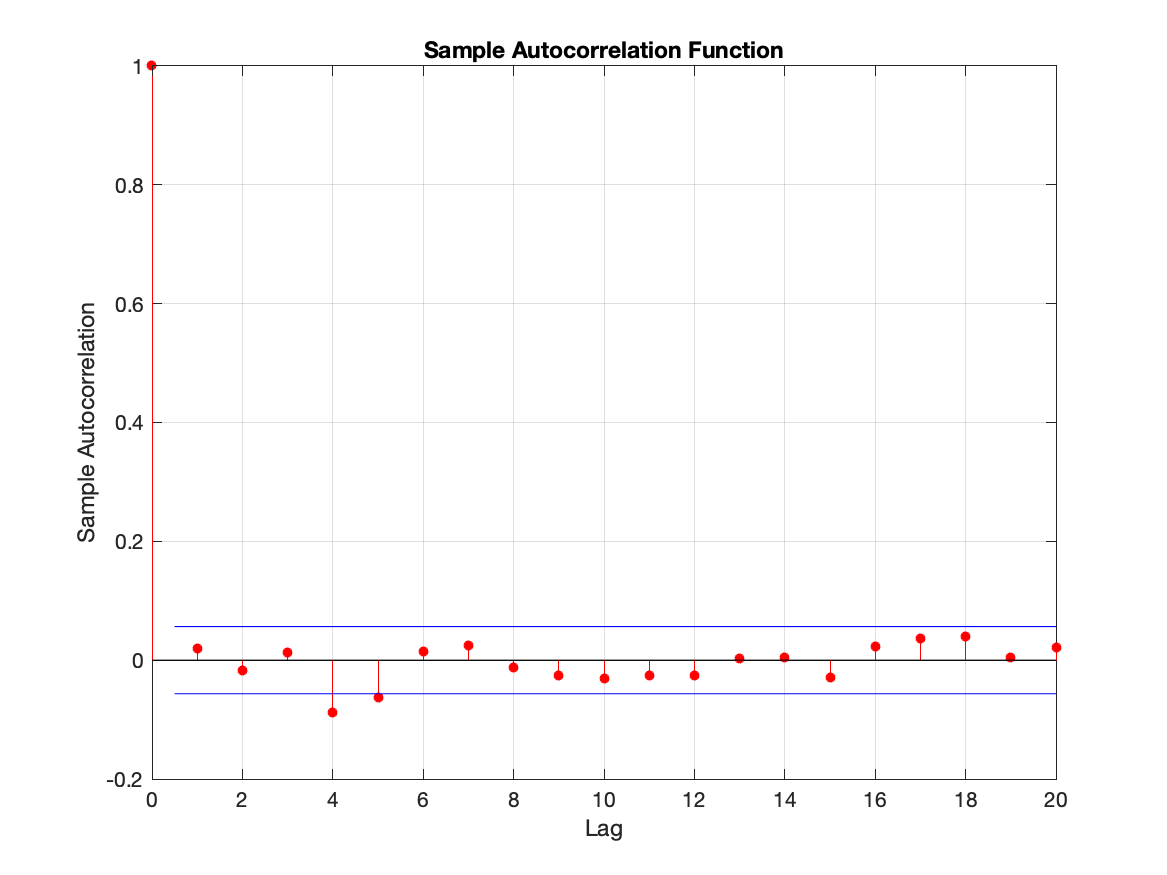
\includegraphics[width=10cm]{plots/acf_log_rtns.png}
\centering
\caption{Autocorrelation function for the log returns}
\label{fig:acf_log_rtns}
\end{figure}

\begin{figure}[H]
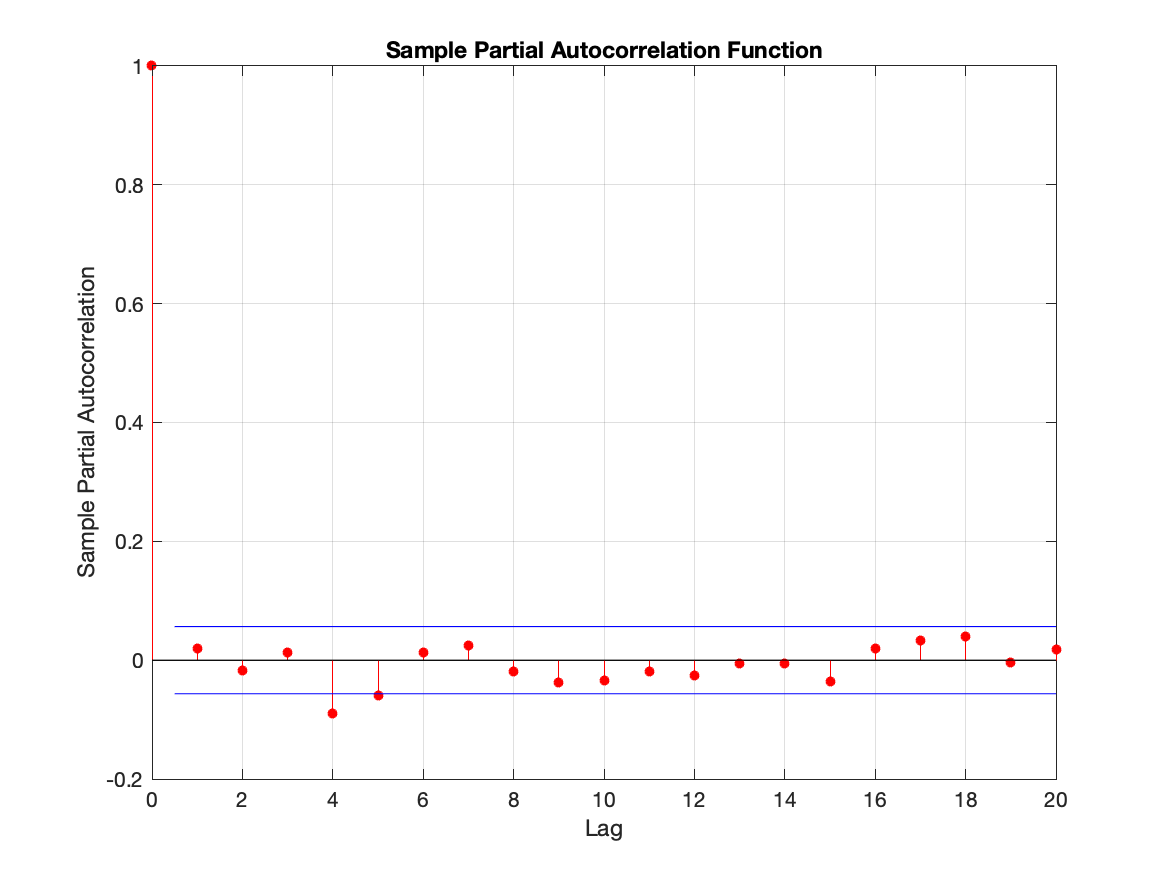
\includegraphics[width=10cm]{plots/pacf_log_rtns.png}
\centering
\caption{Partial autocorrelation function for the log returns}
\label{fig:pacf_log_rtns}
\end{figure}

\begin{figure}[H]
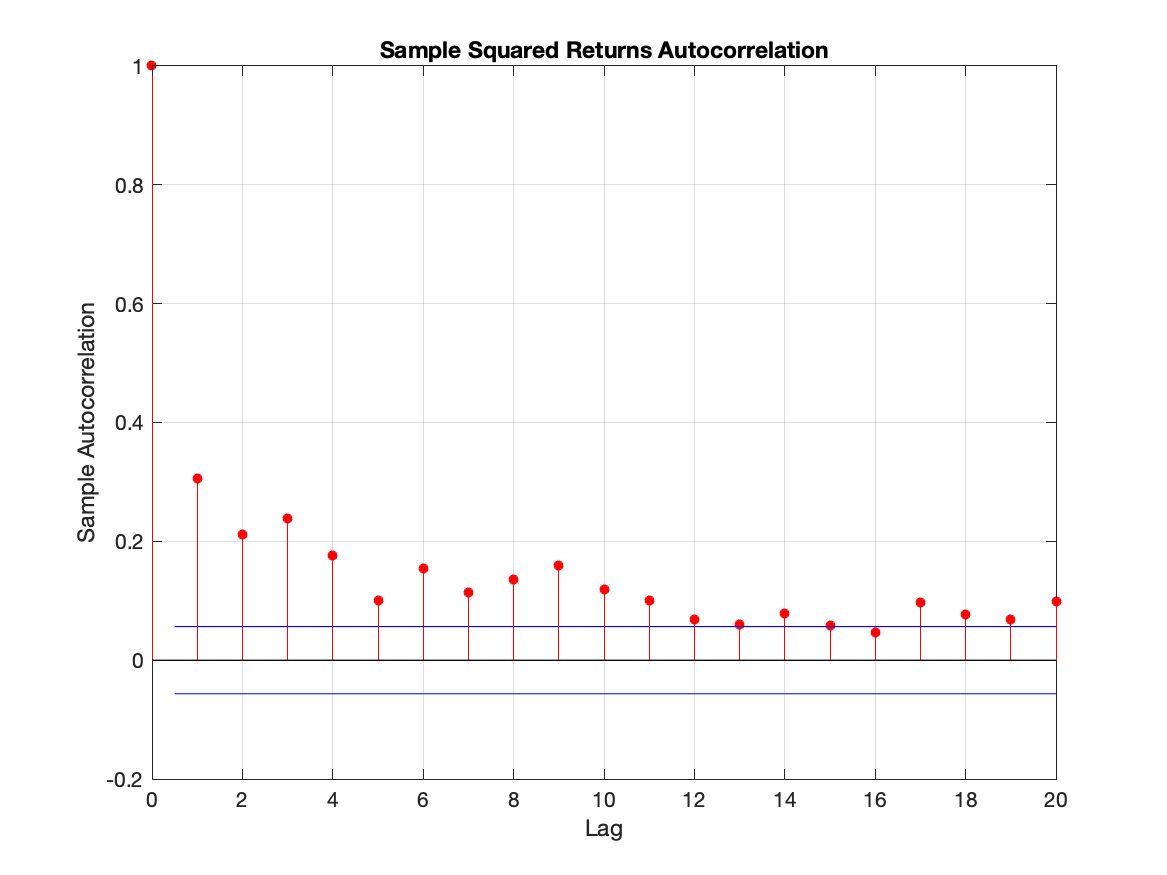
\includegraphics[width=10cm]{plots/acf_square_rtns.png}
\centering
\caption{Autocorrelation function for the squared log returns}
\label{fig:acf_square_rtns}
\end{figure}

\section*{Problem 2}

We split the data into a training set with the first 1000 values and a test set with the remaining data (251 values).
We fit a GARCH(p,q) model with Gaussian errors for each $p = 1, \ldots, 10$ and $q = 1, \ldots, 10$, resulting in 100 different models.
For each of these models we computed the BIC (Bayesian information criteria) and plotted the result in the heatmap shown in Figure \ref{fig:bic_heatmap_norm}.
The minimum model was the GARCH(1,1) model
\begin{align*}
X_t &= \sigma_t Z_t && Z_t \sim IIDN(0, 1)\\
\sigma_t^2 &= \alpha_0 + \alpha_1 X_{t - 1}^2 + \beta_1 \sigma_{t - 1}^2
\end{align*}

\begin{figure}[H]
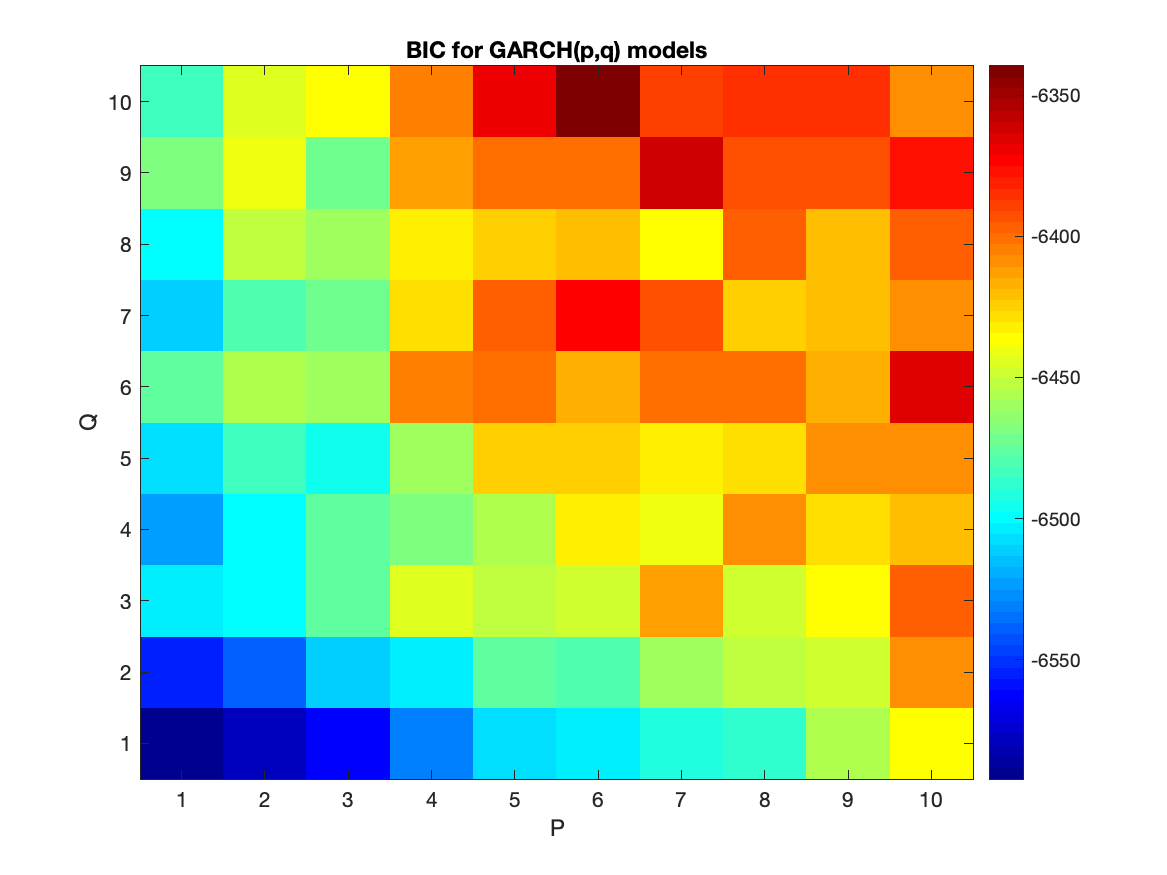
\includegraphics[width=10cm]{plots/bic_heatmap_norm.png}
\centering
\caption{BIC Heatmap for GARCH(p,q) process with Gaussian noise}
\label{fig:bic_heatmap_norm}
\end{figure}

\section*{Problem 3}

Using the GARCH(1,1) model, we computed the residuals:
$$
\hat{R}_t = (X_t - \hat{X_t})/\sqrt{\sigma_t}
$$
and for a GARCH process, $\hat{X}_t = 0$ for all $t \in \mathbb Z$.
We then plotted the residuals (Figure \ref{fig:residual_plots_norm}), QQ plot of the residuals versus standard normal, autocorrelation of residuals, and the autocorrelation of the squared residuals.
The residuals were computed by infering $\hat{\sigma_t}^2$, then dividing the training data by the square root of the infered values, $\hat{\sigma}$.
We would expect these values,
$$
\frac{X_t}{\hat{\sigma}} = Z_t \sim IID(0,1)
$$
Thus, the distribution of the residuals should the residuals should follow a standard normal distribution.
We see that in the QQ plot there is some deviation from the standard normal.
We have heavier tails than we would expect with a standard normal.
The autocorrelation of the sample ACF has almost all of the values within $\pm 1.96 / \sqrt{n}$.
Similarly, the residuals squared also appear to be iid normal as all of the acf values are within $\pm 1.96 / \sqrt{n}$.
Based on the QQ-plot, it makes sense to investigate whether a Student's t distribution, which allows for heavier tails, would fit the data better.

\begin{figure}[H]
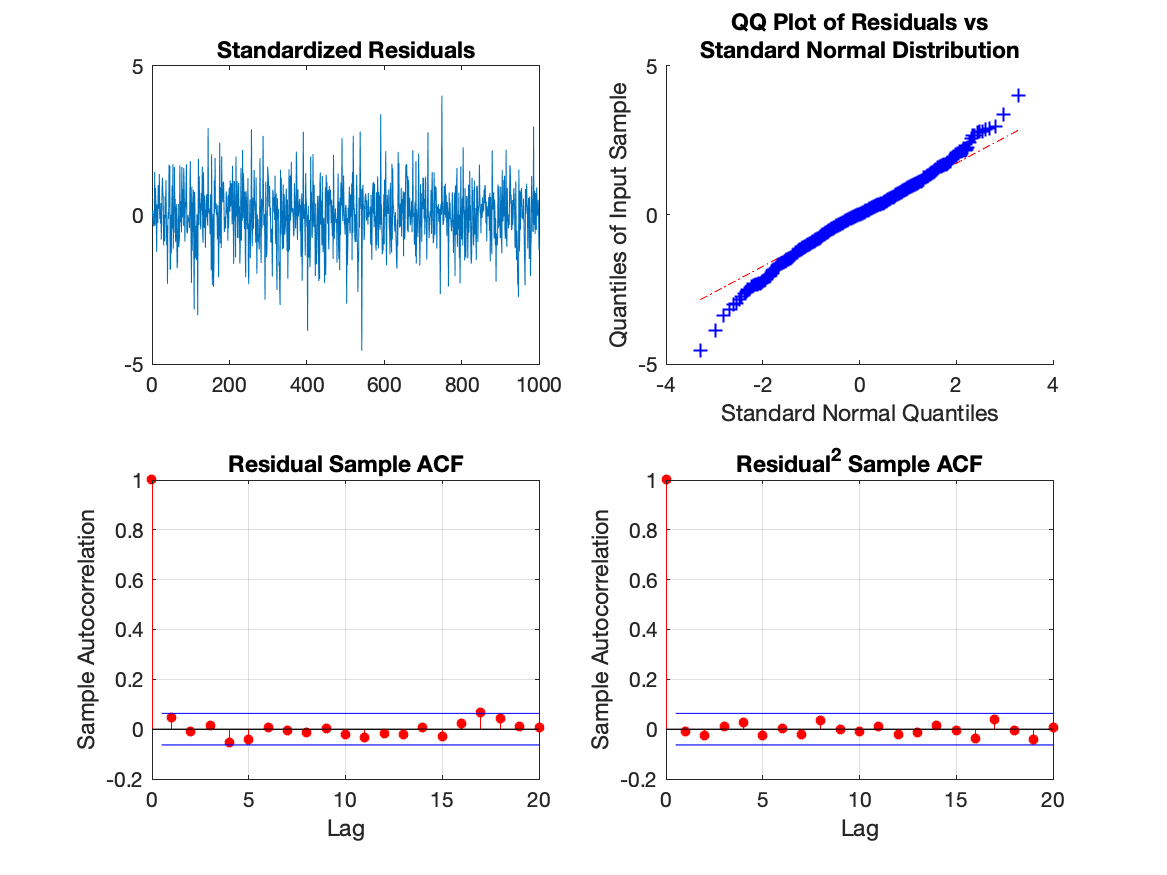
\includegraphics[width=16cm]{plots/residual_plots_norm.png}
\centering
\caption{Residual Plots for GARCH(1,1) process with Gaussian noise}
\label{fig:residual_plots_norm}
\end{figure}

\section*{Problem 4}

Now we have the model

\begin{align*}
X_t &= \sigma_t Z_t && Z_t \sim IIDt(0, 1)\\
\sigma_t^2 &= \alpha_0 + \alpha_1 X_{t - 1}^2 + \beta_1 \sigma_{t - 1}^2
\end{align*}

Where $IID-t(0,1)$ is indepedent and identically distributed Student's t distribution with some degrees of freedom $\nu$.
Again we find that the GARCH(1,1) model has the minimum BIC.
The ACF of the residuals and square residuals are consistent with iid noise as in the previous problem.
A big difference is the QQ plot which now fits almost exactly.
The model was estimated with degrees of freedom equal to 8.03.

\begin{figure}[H]
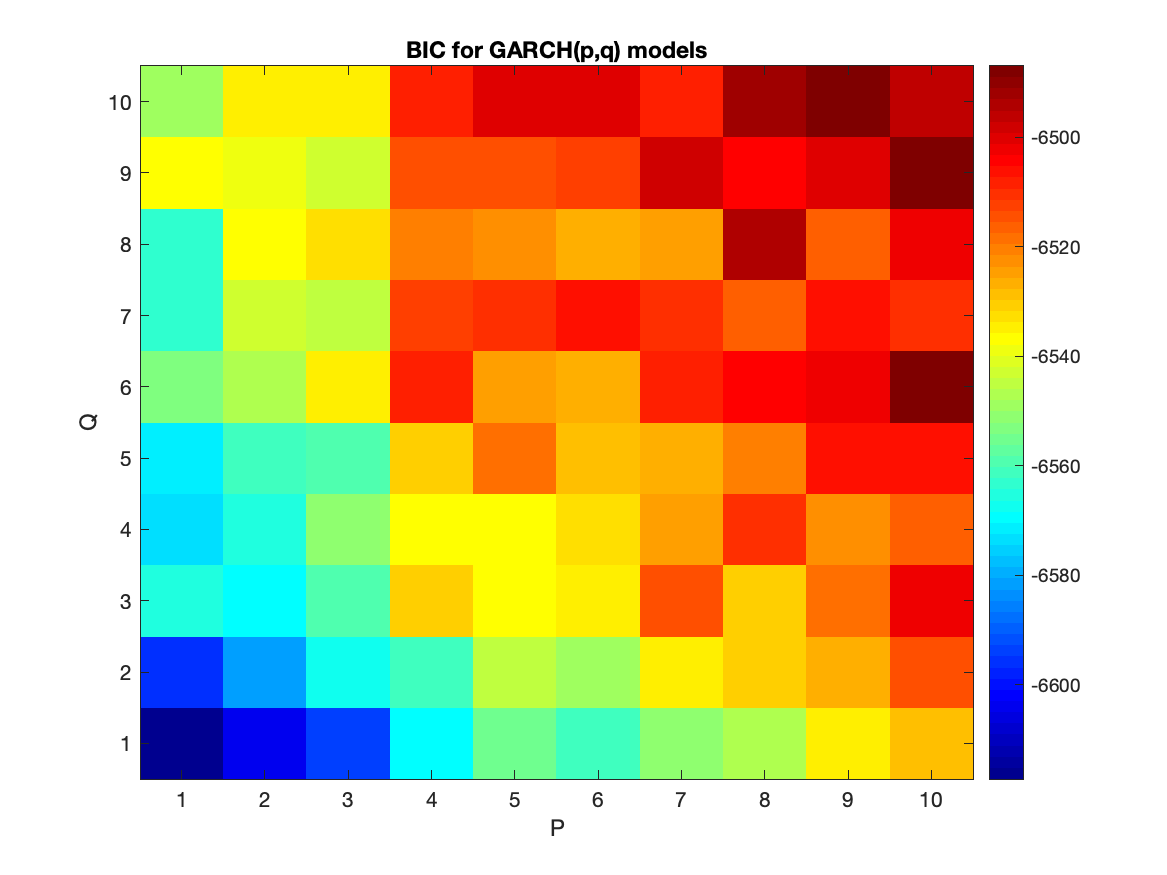
\includegraphics[width=10cm]{plots/bic_heatmap_t.png}
\centering
\caption{BIC Heatmap for GARCH(p,q) process with Student's t distribution noise}
\label{fig:bic_heatmap_t}
\end{figure}

\begin{figure}[H]
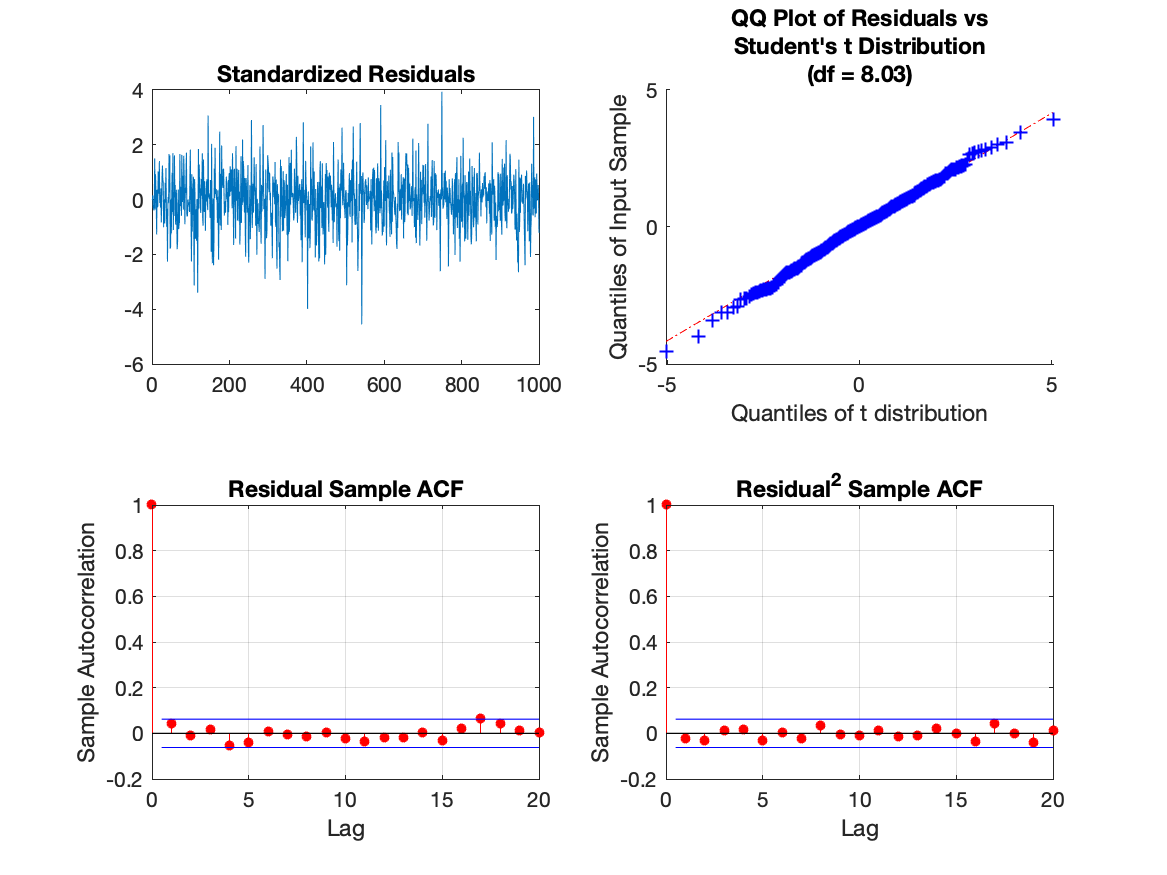
\includegraphics[width=16cm]{plots/residual_plots_t.png}
\centering
\caption{Residual Plots for GARCH(1,1) process with Student's t distribution noise}
\label{fig:residual_plots_t}
\end{figure}

\section*{Problem 5}
The distribution of $X_{t + 1}$ is $N(0, \sigma_{t+1})$ which using the normal errors,
and the distribution is a student's t distribution $t(0, \sigma_{t + 1})$,
where we estimate $\sigma_{t + 1}$ using
$$
\hat{\sigma}_{t + 1} = \hat{\alpha}_0 + \hat{\alpha}_1 X_t^2 + \hat{\beta}_1 \hat{\sigma}_t
$$
This results in confidences intervals
\begin{align*}
&\pm z_{\alpha/2} \cdot \sigma_{t + 1}\\
&\pm t_{\alpha/2, \nu} \cdot \sigma_{t + 1}
\end{align*}
Since we have $\mu = 0$ for $X_{t + 1}$.

We computed the confidence intervals for each $t = 1001,\ldots, 1251$ for both the normal model as well as the t distribution model.
At each step, we used the \textit{forecast} function in matlab and supplied all of the previous values in the log returns $X_t = \log(P_t) - \log(P_{t - 1})$ as the presample innovations.
Also, we computed the simple model which was just the sample variance of the the previous time steps, $X_1, \ldots, X_t$.

\begin{table}[H]
  \centering
\begin{tabular}{l | lll}
& Normal & T & Simple\\ \hline
counts & 250  & 250 & 246 \\
percentage & 0.996 & 0.996 & 0.98   \\
\end{tabular}
\end{table}

\begin{figure}[H]
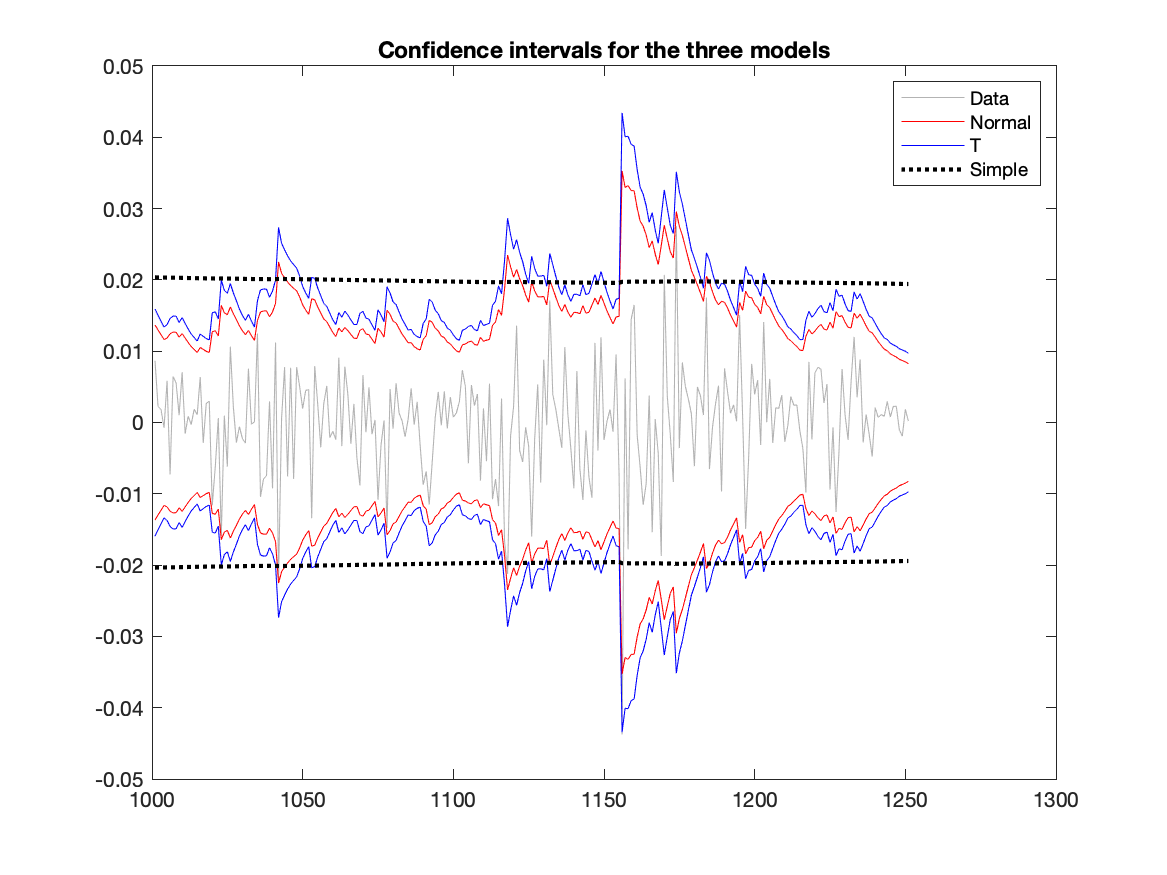
\includegraphics[width=16cm]{plots/conf_ints_overlay.png}
\centering
\caption{Confidence intervals (overlayed) for the three models}
\label{fig:conf_intervals}
\end{figure}

\begin{appendices}

\subsection{project2.m}
\lstinputlisting[language=Octave]{project2.m}

\end{appendices}

%\bibliographystyle{plain}
%\bibliography{references}
\end{document}
